\documentclass{zkdl-presentation-template}

% --- Bitcoin Script helpers ---
\usepackage{etoolbox}
\AtBeginEnvironment{tcolorbox}{\small}
\newtcolorbox{empheqboxed}{
  enhanced,
  boxsep=1pt,
  arc=0.75ex,
  colback=gray!10,
  colframe=gray!40,
  boxrule=1pt,
  leftrule=40pt,
  top=-3.5mm,
  overlay unbroken and first ={%
    \node[minimum width=1cm,
      anchor=south,
      font=\sffamily\bfseries,
      xshift=20pt,
      yshift=-6.5pt,
    black]
    at (frame.west) {\scriptsize Script:};
  }
}

\newcommand{\mycomment}[1]{}
\newcommand{\elem}[1]{\, \langle #1 \rangle \,}
\newcommand{\opcode}[1]{\, \texttt{#1} \,}
\newcommand{\script}[1]{ $\big\{ #1 \big\}$ }

% -- Algorithms --
\usepackage[
    titlenumbered,
    linesnumbered,
    ruled
]{algorithm2e}
\SetKwInOut{Input}{Input}
\SetKwInOut{Output}{Output}
\SetKwInOut{Return}{Return}

% --- Ticks and crosses ---
\usepackage{pifont} % http://ctan.org/pkg/pifont
\newcommand{\cmark}{\textcolor{green!65!black}{\ding{51}}}%
\newcommand{\xmark}{\textcolor{red!80!black}{\ding{55}}}%

% --- Title Page Info ---

\title[BitVM2 Made Practical]{\textbf{$\mathcal{N}\mathfrak{e}\mathcal{R}O$: BitVM2-Based Optimistic Verifiable Computation on Bitcoin}}
\author{Distributed Lab}
\date{October 31, 2024}
\homepage{distributedlab.com/}
\github{distributed-lab/nero}

\begin{document}
    \frame {
        \tikz [remember picture,overlay]
        \node at
            ([yshift=1.5cm,xshift=-1.5cm]current page.south east) 
            %or: (current page.center)
            {
\includegraphics[width=60pt]{icon.png}};
        \titlepage
    }
 
	\begin{frame}{Plan}
        \tableofcontents
    \end{frame}

	\section{Advanced Bitcoin Script}

    \subsection{What is Bitcoin Script? Basic Notation}

    \begin{frame}{What Bitcoin Script is for?}
        \begin{block}{Recall}
            \textbf{Bitcoin Script} is a scripting language used in Bitcoin to specify conditions on how the UTXO can be spent.\pause
        \end{block}

        \begin{example}
            The standard \texttt{pay-to-pubkey-hash} looks as follows. \texttt{scriptPubKey}:
              \begin{empheqboxed}
                \small
                \begin{align*}
                    &\opcode{\texttt{OP\_DUP}} \opcode{\texttt{OP\_HASH160}} \elem{H(\mathsf{pk})} \\ &\opcode{OP\_EQUALVERIFY} 
                    \opcode{OP\_CHECKSIG}
                \end{align*}
              \end{empheqboxed}

            \pause As a \texttt{scriptSig}, the user provides \script{\elem{\sigma} \elem{\mathsf{pk}}}.
        \end{example}
    \end{frame}

    \begin{frame}{How the Bitcoin Script is executed}
        Consider the \texttt{pay-to-pubkey-hash}'s $\texttt{scriptSig} \parallel \texttt{scriptPubKey}$:
      \begin{empheqboxed}
        \scriptsize
        \begin{align*}
            \elem{\sigma} \textcolor{green!50!black}{\elem{\mathsf{pk}'}\opcode{\texttt{OP\_DUP}}} \opcode{\texttt{OP\_HASH160}} \elem{H(\mathsf{pk})} \opcode{OP\_EQUALVERIFY} 
            \opcode{OP\_CHECKSIG}
        \end{align*}
      \end{empheqboxed}\pause
      \begin{empheqboxed}
        \scriptsize
        \begin{align*}
            \elem{\sigma} \elem{\mathsf{pk}'}\textcolor{green!50!black}{\elem{\mathsf{pk}'} \opcode{\texttt{OP\_HASH160}}} \elem{H(\mathsf{pk})} \opcode{OP\_EQUALVERIFY} 
            \opcode{OP\_CHECKSIG}
        \end{align*}
      \end{empheqboxed}\pause
      \begin{empheqboxed}
        \scriptsize
        \begin{align*}
            \elem{\sigma} \elem{\mathsf{pk}'}\textcolor{green!50!black}{\elem{H(\mathsf{pk}')} \elem{H(\mathsf{pk})} \opcode{OP\_EQUALVERIFY}}
            \opcode{OP\_CHECKSIG}
        \end{align*}
      \end{empheqboxed}\pause
      \begin{empheqboxed}
        \scriptsize
        \begin{align*}
            \textcolor{green!50!black}{\elem{\sigma} \elem{\mathsf{pk}'}
            \opcode{OP\_CHECKSIG}}
        \end{align*}
      \end{empheqboxed}\pause
      \begin{empheqboxed}
        \scriptsize
        \begin{align*}
            \elem{1}
        \end{align*}
      \end{empheqboxed}\pause

      \begin{block}{Note}
          One can spend the UTXO iff the output is \texttt{OP\_1}. 
      \end{block}
    \end{frame}

    \subsection{Non-Native Verifications}
    \begin{frame}{Can we do more?}
        So typically, Bitcoin Script allows writing only basic smart contracts using \textbf{native} \texttt{OP\_CODE}s: 
        \begin{itemize}[label=\cmark]
            \item Hash Preimage Verification and Timelocks.\pause
            \item Basic Signatures (ECDSA for tx data, Schnorr for Taproot).\pause
            \item Threshold/Multisignatures.\pause
            \item Combination of those.\pause
        \end{itemize}

        \begin{alertblock}{Question}
            Can we implement some non-native verifications? For example, zk-SNARKs (Groth16, fflonk), zk-STARKs, BLS Signatures?
        \end{alertblock}
    \end{frame}

    \begin{frame}{Can we do more?}
        \begin{itemize}[label={}]
            \item \cmark \hspace{1px} Groth16 is already implemented.\pause
            \item \cmark \hspace{1px} \textsf{fflonk} is already implemented.\pause
            \item \xmark \hspace{1px} zk-STARK cannot be currently implemented (requires \texttt{OP\_CAT} for Fiat-Shamir transformation and Merkle Trees). Yet, assuming \texttt{OP\_CAT}, the \href{https://eprint.iacr.org/2024/278}{\textcolor{blue!70!white}{\textbf{Circle STARK}}} is implemented!\pause
            \item \cmark \hspace{1px} Any discrete-log-based protocol that does not involve hashing (typically requiring concatenation) can be implemented: $\Sigma$-protocols, Bulletproofs, BLS Signatures.\pause
        \end{itemize}

        \begin{block}{Note}
            In other words, currently, it is \textit{theoretically possible} to build a Groth16 zk-SNARK verification of proof $\pi$ in a form
            \begin{empheqboxed}
            \small
            \begin{align*}
                \elem{\pi} \elem{\textsf{public statement}} \opcode{OP\_CHECKGROTH16}
            \end{align*}
          \end{empheqboxed}
        \end{block}
    \end{frame}

    \subsection{Demystifying Math behind BitVM Groth16}
    
    \begin{frame}{Demystifying Math behind BitVM Groth16}
        \begin{itemize}[label=\cmark]
            \item Arithmetic is allowed only over \texttt{u32} integers.\pause
            \item From arithmetic, one only\footnote{With dropping variations such as \texttt{OP\_1ADD} and such.} has \texttt{OP\_ADD}, \texttt{OP\_SUB}, \texttt{OP\_NEGATE}, \texttt{OP\_ABS}, \texttt{OP\_LESSTHAN}, \texttt{OP\_GREATERTHAN}, \texttt{OP\_BOOLAND}, \texttt{OP\_BOOLOR}.\pause
            \item Flow control is very limited: only \texttt{OP\_IF}s/\texttt{OP\_ELSE}s are allowed. No for/while loops, but almost full control of compile-time stack movement.\pause
        \end{itemize}

        \begin{alertblock}{Question}
            (Almost) any zk-SNARK requires working over large finite fields (with a bit-size of $254$). How do we even push a 254-bit big integer?
        \end{alertblock}
    \end{frame}

    \begin{frame}{Representing large integers}
        \begin{block}{Recall}
            We can represent any integer $x$ in arbitrary base $b$:
            \begin{equation*}
                x = \sum_{j=0}^{n-1} x_jb^j, \quad 0 \leq x_j < b
            \end{equation*}
            \pause Numbers $x_0,x_1,\dots,x_{n-1}$ are called \textbf{limbs}, where $n$ is the \textbf{limb-size} of $x$ in base $b$.\pause
        \end{block}

        \begin{alertblock}{Idea \#1}
            If $b$ is small enough, we can publish individual limbs $x_0,\dots,x_{n-1}$ that constitute the whole number $x$.\pause
        \end{alertblock}

        \begin{alertblock}{Idea \#2}
            Since we want to minimize the number of limbs, we take the largest $b$ possible (with $b=2^t$ for convenience). Thus, we set $b := 2^{30}$.
        \end{alertblock}
    \end{frame}

    \begin{frame}{Representing large integers}
        \begin{example}
            Consider the following 254-bit integer:
            \begin{align*}
                x &= (\mathtt{0xbe48fffd2a6f534dc} \\ &\mathtt{5b6a6901840fc0fb65827e6} \\
                &\mathtt{efd22a8063cded681f5f7b2})
            \end{align*}
            \pause To add this integer to the stack, one uses the following script:
            \begin{empheqboxed}
            \scriptsize
            \begin{align*}
               &\opcode{OP\_PUSHBYTES\_2} \elem{\mathtt{e40b}} \opcode{OP\_PUSHBYTES\_4} \elem{\mathtt{a9f4ff23}}
               \\ 
               &\opcode{OP\_PUSHBYTES\_4} \elem{\mathtt{c54d532f}} \opcode{OP\_PUSHBYTES\_4} \elem{\mathtt{06a4a92d}}
               \\
               &\opcode{OP\_PUSHBYTES\_4} \elem{\mathtt{fbc00f04}} \opcode{OP\_PUSHBYTES\_4} \elem{\mathtt{9b9f6019}}
               \\
               &\opcode{OP\_PUSHBYTES\_4} \elem{\mathtt{802ad22f}} 
               \opcode{OP\_PUSHBYTES\_4} \elem{\mathtt{5a7bf318}}
               \\
               &\opcode{OP\_PUSHBYTES\_4} \elem{\mathtt{b2f7f501}}
            \end{align*}
          \end{empheqboxed}
          \pause \textbf{Note}: One needs \textbf{9 limbs} to represent a 254-bit integer.
        \end{example}
    \end{frame}

    \begin{frame}{BigInt Addition}
        \begin{block}{Problem}
            Given two 254-bit integers $x$ and $y$, find $z := x+y$, assuming overflowing does not occur.\pause
        \end{block}

        \textbf{Solution.} We have two representations:
        \begin{equation*}
            x = \sum_{j=0}^8 x_j \times 2^{30j}, \quad y = \sum_{j=0}^8 y_j \times 2^{30j}
        \end{equation*}

        \pause \textbf{Idea:} add limb by limb, starting from the least significant one.\pause

        \begin{enumerate}
            \item On step $i$, calculate $t \gets x_i + y_i + \mathsf{carry}$ (start with zero carry).\pause
            \item If $t < 2^{30}$, set $z_i \gets t$, $\mathsf{carry} \gets 0$.\pause
            \item If $t \geq 2^{30}$, set $z_i \gets t-2^{30}$, $\mathsf{carry} \gets 1$.
        \end{enumerate}
    \end{frame}

    \begin{frame}{BitInt Addition: Bitcoin Script}
        \begin{figure}
            \centering
            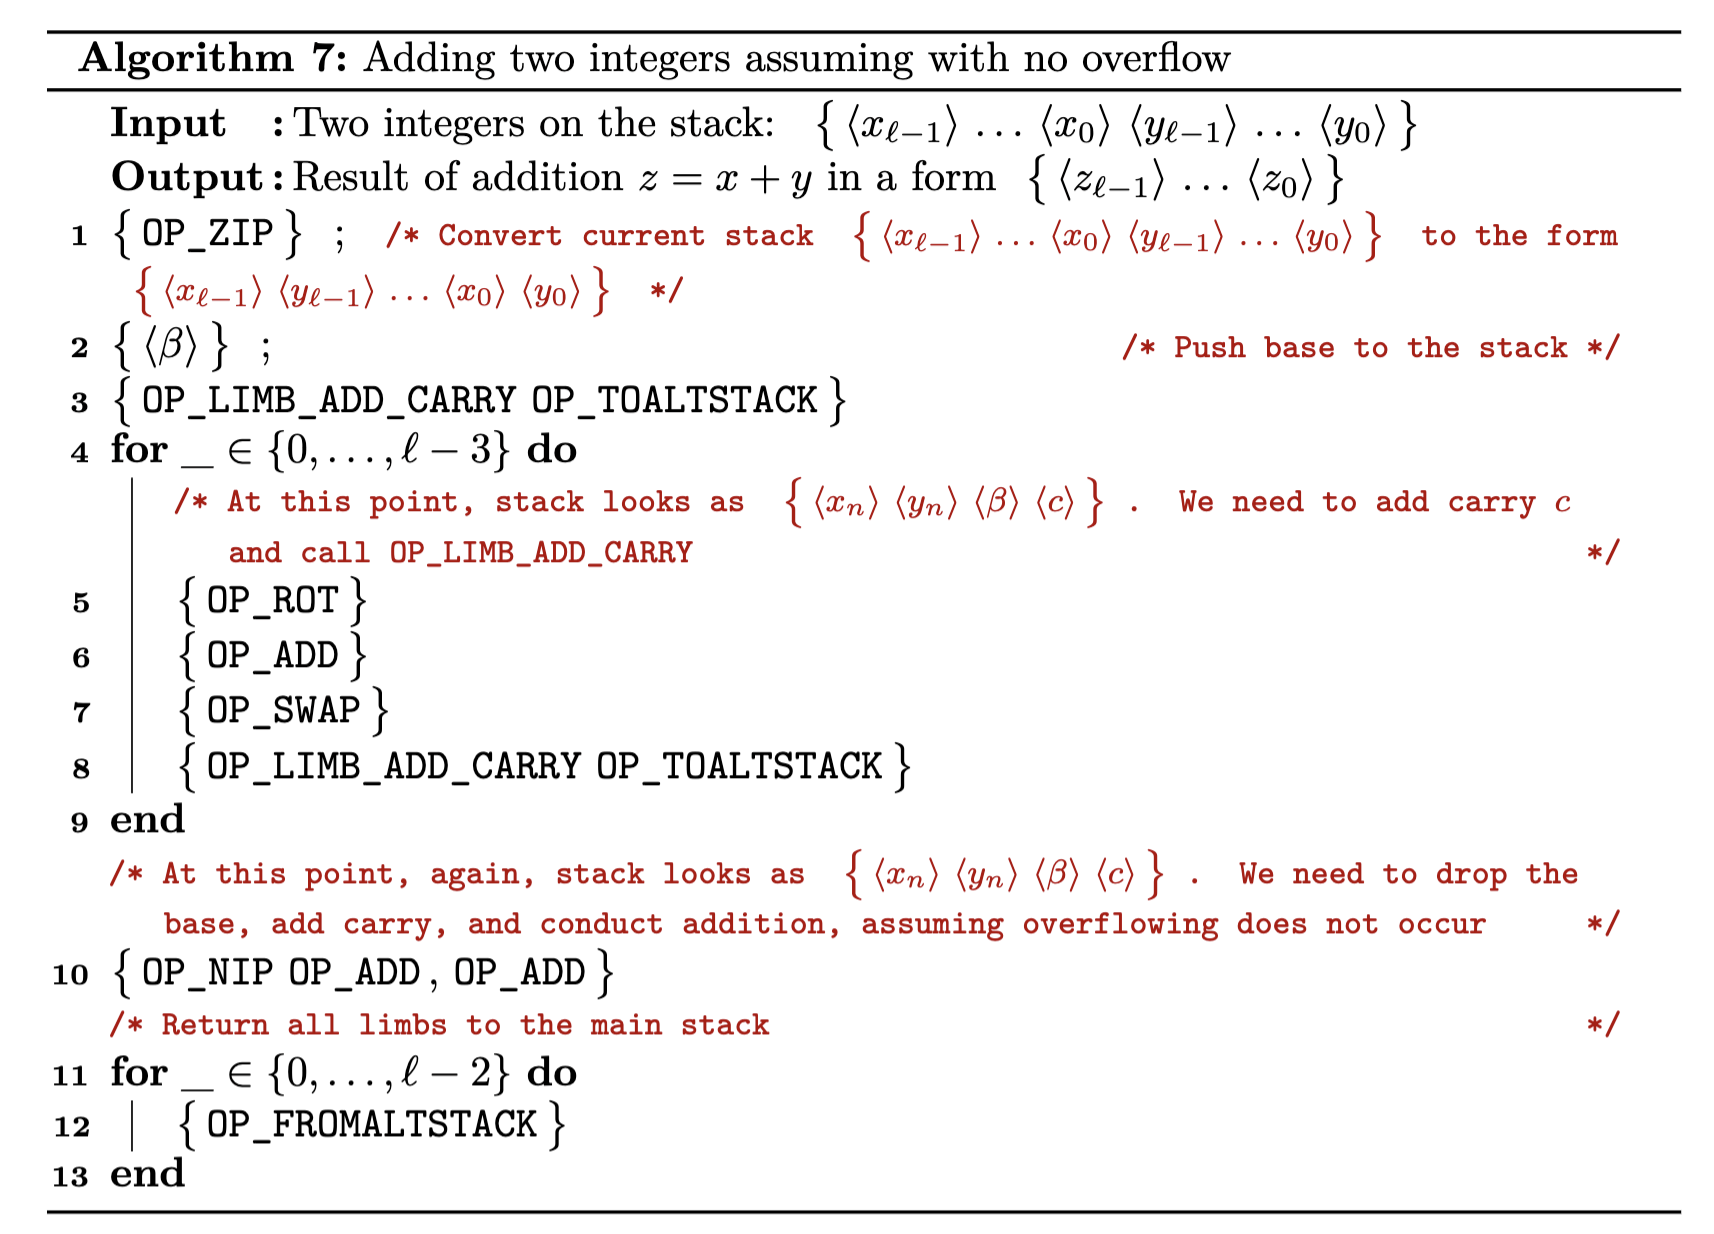
\includegraphics[width=\linewidth]{images/bigint_add.png}
        \end{figure}
    \end{frame}

    \begin{frame}[fragile]{BigInt Multiplication}
        \begin{block}{Problem}
            Given two 254-bit integers $x$ and $y$, find 508-bit $z := x \times y$.\pause
        \end{block}

        \small
        \begin{algorithm}[H]
          \caption{Double-and-add method for integer multiplication}\label{alg:double_and_add}
          \Input{$x,y$ --- two integers being multiplied}
          \Output{Result of the multiplication $x \times y$}
          
          Decompose $y$ to the binary form: $(y_0,y_1,\dots,y_{N-1})_2$\pause
          
          $r \gets 0$
          
          $t \gets x$\pause
          
          \For{$i \in \{0,\dots,N-1\}$}{
              \If{$y_i = 1$}{
                  $r \gets r + t$
              }
          
              $t \gets 2 \times t$
          }\pause
          
          \Return{Integer $r$}
          
        \end{algorithm}
    \end{frame}

    \begin{frame}[fragile]{Other Primitives to Implement\ldots}
        \begin{figure}
            \centering
            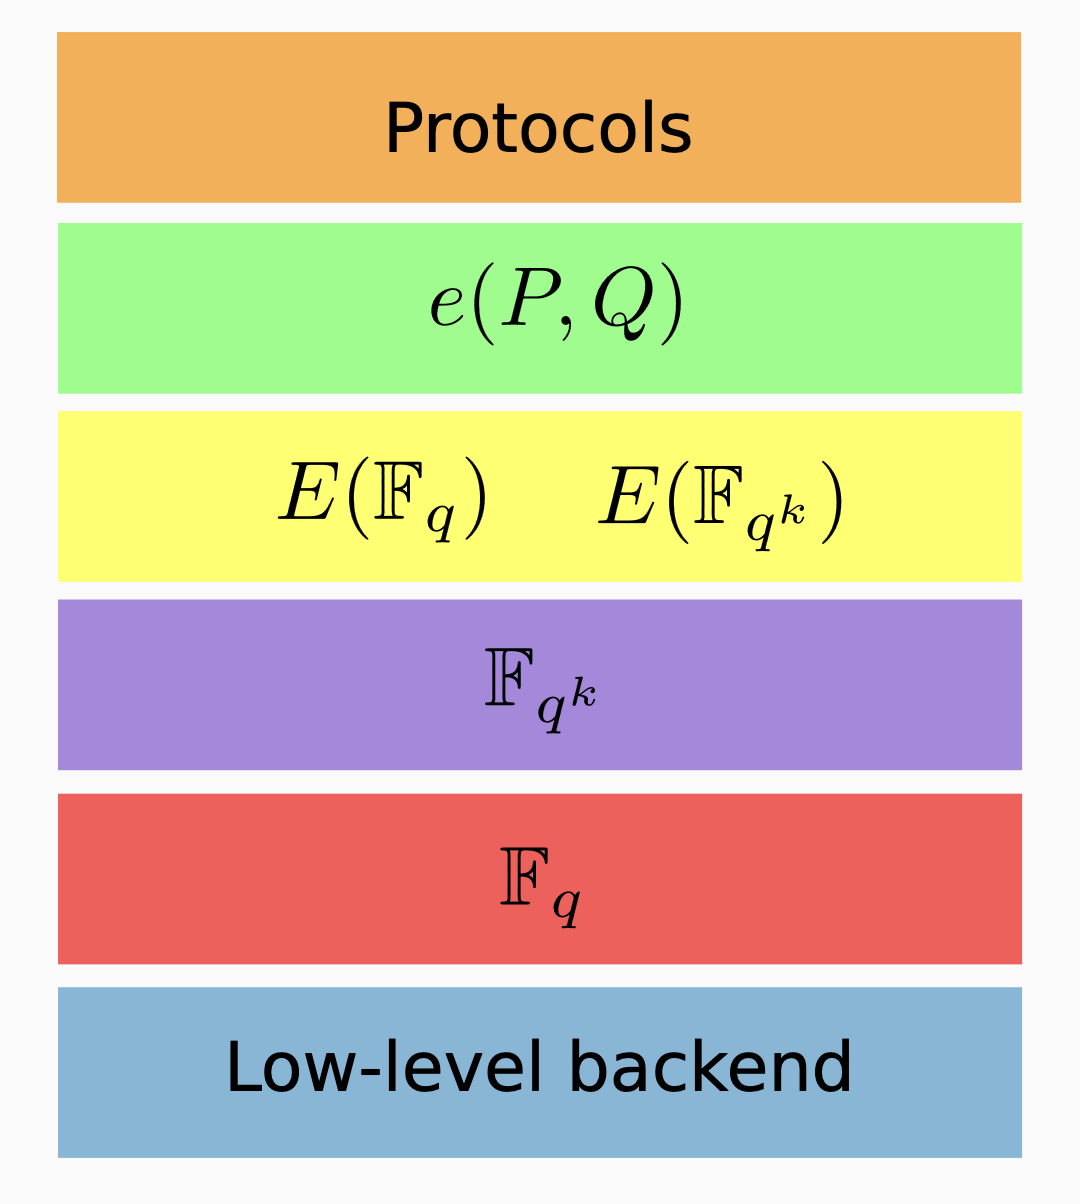
\includegraphics[width=0.575\linewidth]{images/levels.png}
            \caption{Primitives to implement}
            \label{fig:primitives}
        \end{figure}
    \end{frame}

    \begin{frame}{What is the problem then?}
        If Groth16 is already implemented, what is the reason we are here?\pause

        The thing is\ldots Currently, fflonk verification script is \textbf{875MB} in size, while Groth16 takes \textbf{1.3GB} (after \href{https://eprint.iacr.org/2024/1236}{\textcolor{blue!70!white}{our and Alpen Labs optimization}} using $w$-window multiplication)\ldots See \href{https://x.com/fiamma_chain/status/1830824142826086608?s=46}{\textcolor{blue!70!white}{this post}} for more details.

        The current Bitcoin mainnet restriction is roughly 4MB (while the practical limitation is about 200-400kB). What to do?

        \begin{figure}
            \centering
            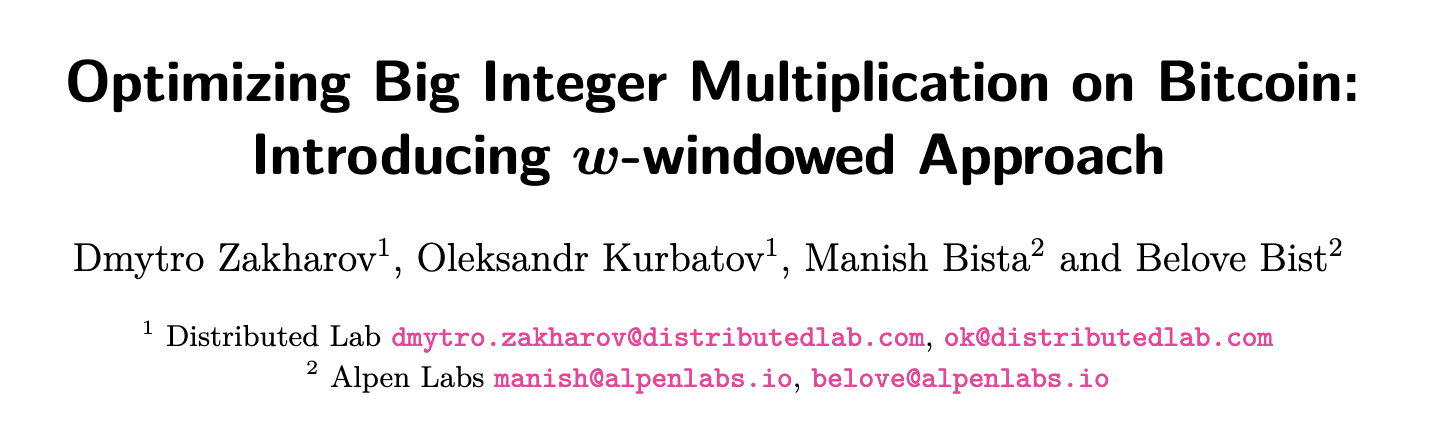
\includegraphics[width=\linewidth]{images/w_mul.png}
            \caption{Our paper on optimizing big integer multiplication}
            \label{fig:w_mul}
        \end{figure}
    \end{frame}

    \begin{frame}[plain, standout]
        \centering
        \LARGE
        \textbf{Questions before moving on?}
    \end{frame}

    \section{BitVM2}

    \subsection{Shard Splitting}

    \begin{frame}{Core Idea}
        Suppose our script is represented as a function $f$. Our input (\texttt{ScriptSig}/\texttt{witness}) is $x$, while the output is $y=f(x)$.\pause

        \begin{block}{Note}
            Although BitVM2's primary goal is implementing the Groth16 verifier (so $f$ is the ZKP verification function), we believe the concept is easily generalizable to any $f$.\pause
        \end{block}
    
        \begin{block}{Idea \#1}
            We do not need to compute $y$ from $x$. Instead, the \textbf{operator} publishes $x$, $y$ ($f$ is publically known as the part of the protocol), and if $y \neq f(x)$, anyone can punish the operator.\pause
        \end{block}

        \begin{alertblock}{?!}
            However, doesn't check $y \neq f(x)$ involve calculating $f$ as a whole?
        \end{alertblock}
    \end{frame}

    \begin{frame}{Shards Splitting}
        \begin{block}{Idea \#2}
            We can ease the challenger's burden by \textbf{splitting the function $f$ into subchunks}. In other words, suppose $f=f_n \circ f_{n-1} \circ \dots \circ f_1$. Then, the operator can calculate the \textbf{intermediate states}:
            \begin{equation*}
                z_1 = f_1(z_0), \; z_2 = f_2(z_1), \; z_3 = f_3(z_2), \dots, \; z_n = f_n(z_{n-1})
            \end{equation*}
            Where $z_0$ is $x$ and $z_n$ \textbf{must} be $y$.\pause
        \end{block}

        \begin{block}{Idea \#3}
            If $y \neq f(x)$, that means that for some shard, $z_{j} \neq f_{j}(z_{j-1})$.\pause
        \end{block}

        \begin{block}{Why this is useful?}
            \begin{itemize}[label=\cmark]
                \item Disproving $z_j \neq f_j(z_{j-1})$ is \textbf{much} easier than $y \neq f(x)$.\pause
                \item For stack-based languages, $f_1 \circ f_2 = f_2 \parallel f_1$.
            \end{itemize}
        \end{block}
    \end{frame}

    \begin{frame}{Shards Splitting: Example}
        \begin{example}
            Consider a fairly simple program $f$:
            \begin{equation*}
                f(a,b) = 25a^2b^2(a+b)^2
            \end{equation*}

            \pause Its implementation (assuming \texttt{OP\_MUL} is implemented):
            \begin{empheqboxed}
                \small
                \begin{align*}
                    &\elem{a} \elem{b} \opcode{\texttt{OP\_2DUP}} \opcode{\texttt{OP\_ADD}} \opcode{\texttt{OP\_MUL}} \opcode{\texttt{OP\_MUL}} 
                    \opcode{\texttt{OP\_DUP}} \opcode{\texttt{OP\_DUP}} \\& \opcode{\texttt{OP\_ADD}} \opcode{\texttt{OP\_DUP}} \opcode{\texttt{OP\_ADD}} \opcode{\texttt{OP\_ADD}} \opcode{\texttt{OP\_DUP}} \opcode{\texttt{OP\_MUL}}
                \end{align*}
            \end{empheqboxed}

            \pause Let us split the function into three shards $\textcolor{red!80!white}{f_1}$, $\textcolor{blue}{f_2}$, and $\textcolor{green!60!black}{f_3}$:
            \begin{align*}
                \textcolor{red!80!white}{f_1}(x,y) = xy(x+y), \quad \textcolor{blue}{f_2}(z) = 5z, \quad \textcolor{green!60!black}{f_3}(w) = w^2
            \end{align*}
        \end{example}
    \end{frame}
  
  \begin{frame}{Shards Splitting: Example (cont.)}  
    \begin{example}
        This way, it is fairly easy to see that $f(a,b) =
    \textcolor{green!60!black}{f_3} \circ \textcolor{blue}{f_2} \circ
    \textcolor{red!80!white}{f_1}(a,b)$. In turn, in Bitcoin script we can
    represent $f$ as $\textcolor{red!80!white}{f_1} \parallel
    \textcolor{blue}{f_2} \parallel \textcolor{green!60!black}{f_3}$:
        \begin{empheqboxed}
            \scriptsize
            \begin{align*}
                &\elem{a} \elem{b} \textcolor{red!80!white}{\opcode{\texttt{OP\_2DUP}} \opcode{\texttt{OP\_ADD}} \opcode{\texttt{OP\_MUL}} \opcode{\texttt{OP\_MUL}}} && \textcolor{gray!80!black}{\text{// $xy(x+y)$}} \\
                &\textcolor{blue}{\opcode{\texttt{OP\_DUP}} \opcode{\texttt{OP\_DUP}} \opcode{\texttt{OP\_ADD}} \opcode{\texttt{OP\_DUP}} \opcode{\texttt{OP\_ADD}} \opcode{\texttt{OP\_ADD}}} && \textcolor{gray!80!black}{\text{// $5z$}} \\
                &\textcolor{green!60!black}{\opcode{\texttt{OP\_DUP}} \opcode{\texttt{OP\_MUL}}}&&\textcolor{gray!80!black}{\text{// $w^2$}}
            \end{align*}
        \end{empheqboxed}
        \pause Suppose $a=2$, $b=3$. Then, intermediate states are:
        \begin{align*}
            & z_0 = (2,3) && \textcolor{gray!80!black}{\text{// Script input}} \\
            & z_1 = f_1(z_0) = 2 \times 3 \times (2+3) = 30 && \\ 
            & z_2 = f_2(z_1) = 5 \times 30 = 150 && \\
            & z_3 = f_3(z_2) = 150^2 = 22500 && \textcolor{gray!80!black}{\text{// Script output}}
        \end{align*}
    \end{example}
  \end{frame}

    \subsection{Protocol}
      \begin{frame}{Naive Version}  
        \begin{enumerate}
            \item Operator splits the program $f$ into shards $f_1,\dots,f_n$ with intermediate states $z_0,\dots,z_n$ and commitments $\sigma_0,\dots,\sigma_n$.
            \item Operator creates an \textbf{Assert Transaction} that can be spent in $n+1$ different ways (taptree):
            \begin{itemize}[label={}]
                \item $((j+1)^{\text{th}})$ \hspace{1px} \textbf{DisproveScript}\texttt{[}$j$\texttt{]}: Challenger shows $z_{j+1} \neq f_j(z_j)$.
                \item ($(n+1)^{\text{th}}$) \hspace{1px} \textbf{Payout}: \texttt{LockTimeVerify} + \texttt{CheckSig}.
            \end{itemize}
        \end{enumerate}

        \begin{figure}
            \centering
            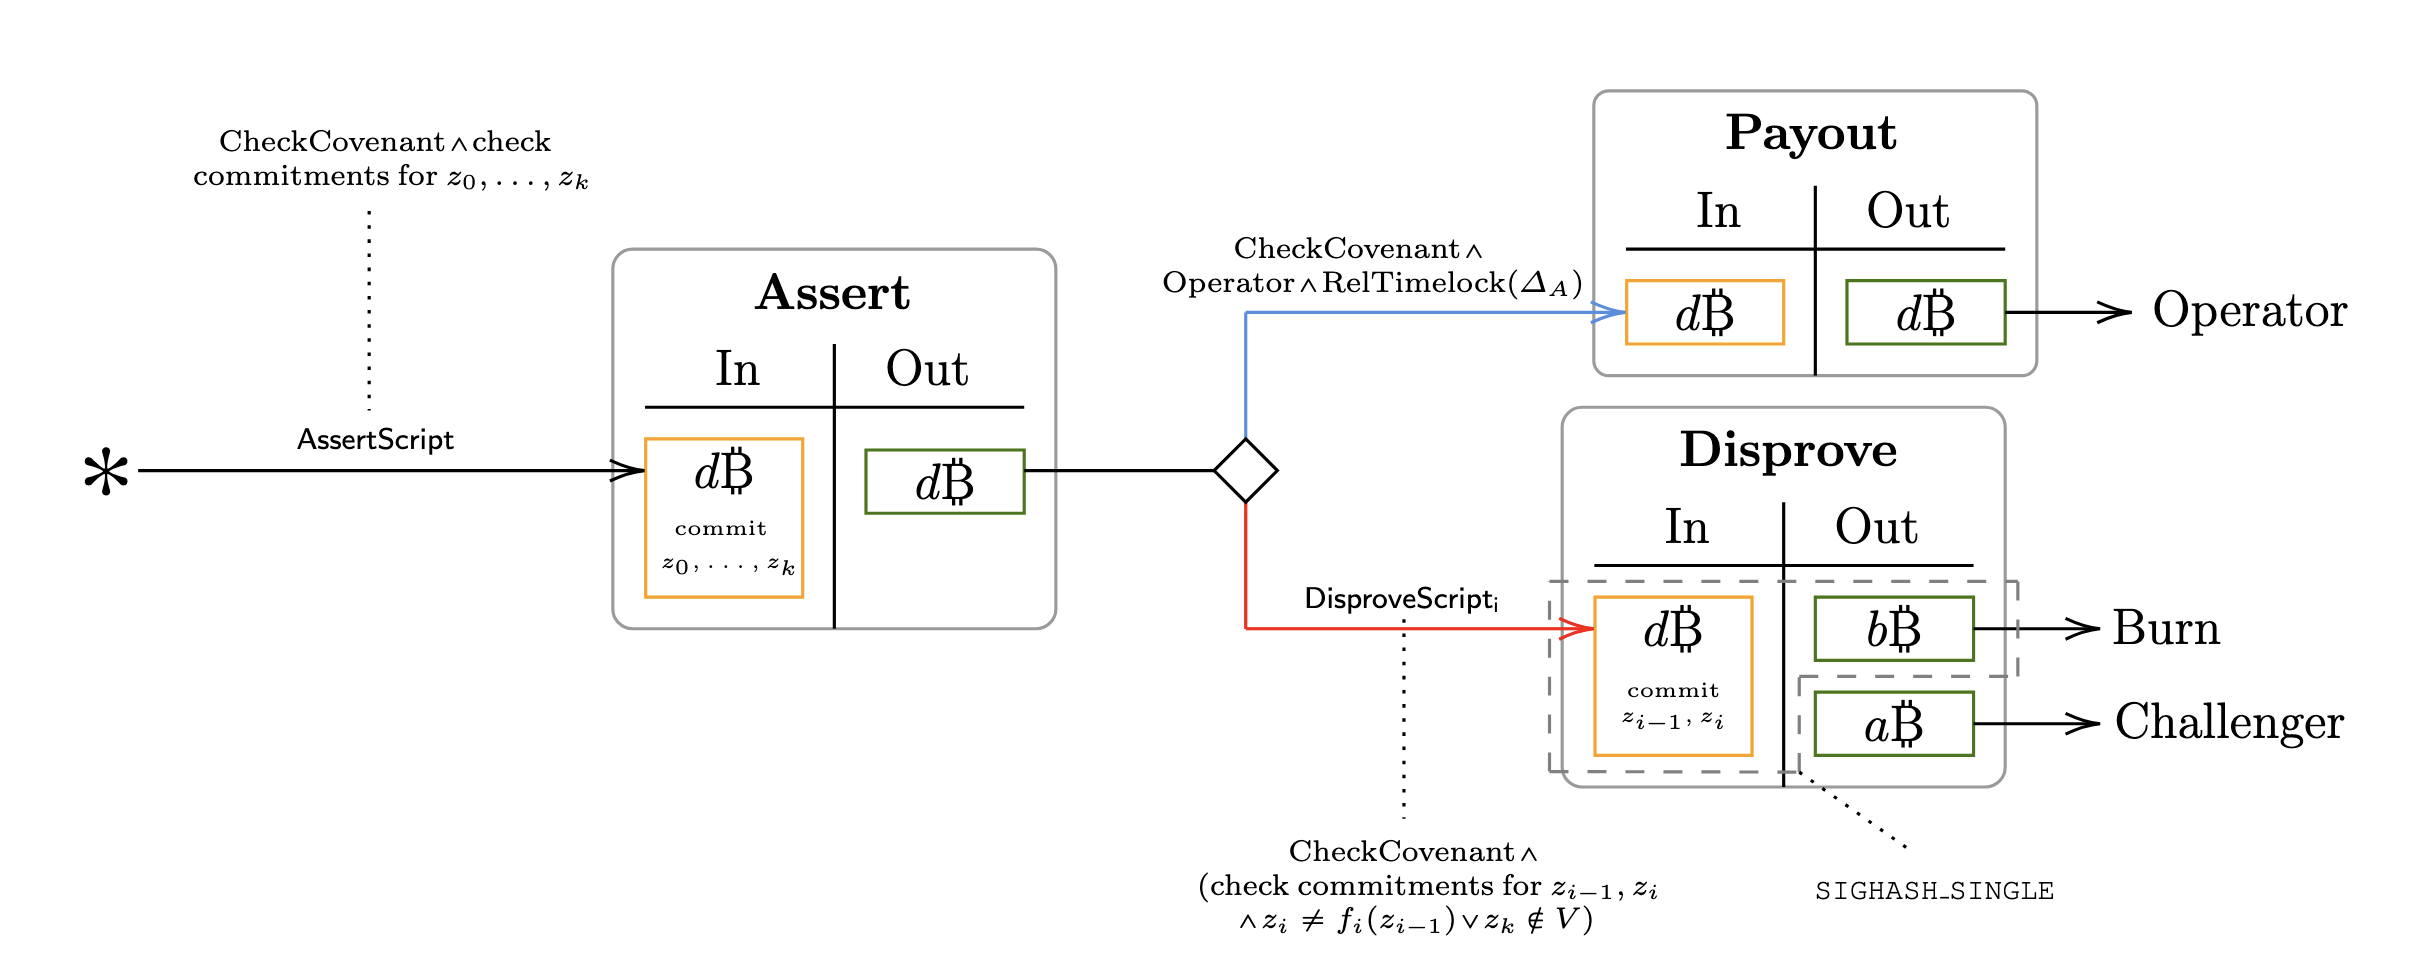
\includegraphics[width=0.95\linewidth]{images/bitvm_basic_structure.png}
            \caption{BitVM2 Naive Version from the original paper}
            \label{fig:bitvm2_naive}
        \end{figure}
      \end{frame}

      \begin{frame}{``Super-Optimistic'' Version}  
        Operator creates a \textbf{Claim Tx} with commitments, and Challenger publishes the \textbf{Challenge Tx} in case of suspicion. Rest is the same.

        \begin{figure}
            \centering
            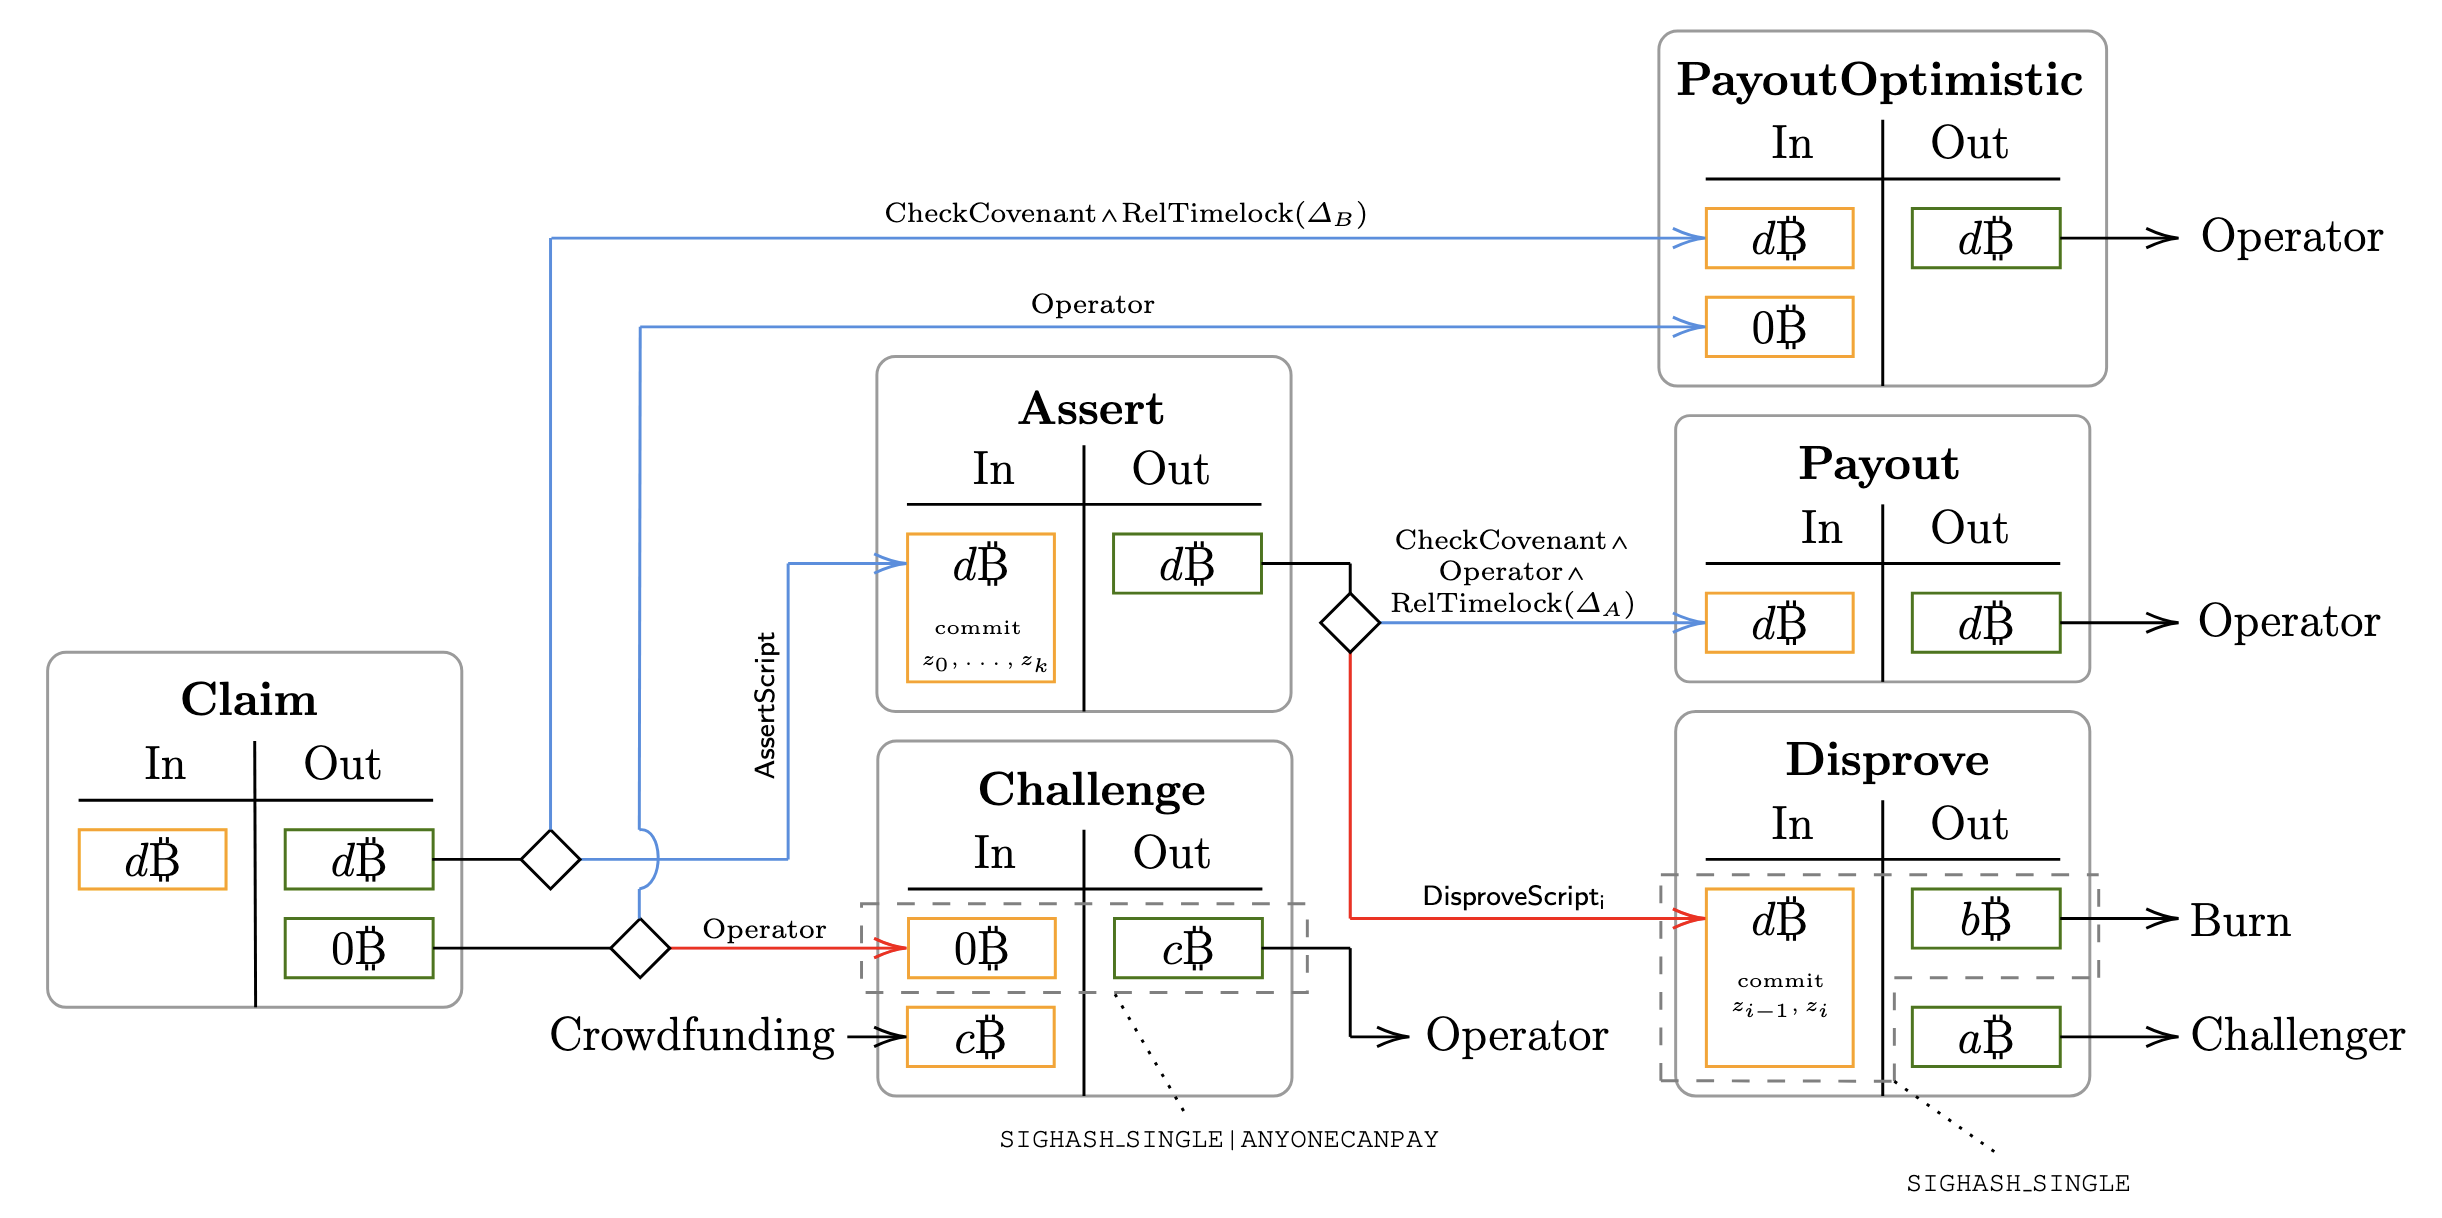
\includegraphics[width=\linewidth]{images/bitvm_optimized.png}
            \caption{BitVM2 Optimized Version from the original paper}
            \label{fig:bitvm2_optimized}
        \end{figure}
      \end{frame}

    \section{BitVM2 Pitfalls}

    \subsection{Splitting Mechanism}

     \begin{frame}{Main Problem}
        How do we implement the \texttt{DisproveScript}?\pause

        \begin{empheqboxed}
          \begin{align*}
            &\elem{z_{j-1}} \opcode{OP\_DUP} \elem{\sigma_{j-1}}
            \elem{\mathsf{pk}_{j-1}} \opcode{OP\_WINTERNITZVERIFY} \\
            &\elem{z_{j}} \opcode{OP\_DUP} \elem{\sigma_{j}}
            \elem{\mathsf{pk}_{j}} \opcode{OP\_WINTERNITZVERIFY} \\
            &\elem{f_j} \opcode{OP\_EQUAL} \opcode{OP\_NOT}
          \end{align*}
        \end{empheqboxed}

        \pause $\mathsf{pk}$'s and $z$'s are stored in the \texttt{scriptPubKey}, while $\sigma$'s (Winternitz signatures) are provided by the challenger in the \texttt{witness}.\pause

        \begin{alertblock}{Main Problem}
            \begin{enumerate}
                \item Each $z_j$ is a collection of \texttt{u32} elements.\pause
                \item This collection cannot be aggregated (e.g., $H(z_{j,1} \parallel z_{j,2} \parallel \dots )$).\pause
                \item Thus, every stack element must be signed separately.\pause
                \item Signing each element costs roughly 1kB \textcolor{red!70!black}{(!!!)}
            \end{enumerate}
        \end{alertblock}
    \end{frame}
    
    \begin{frame}{Splitting}
        Now, how do we actually implement splitting?\pause

        \begin{block}{Idea \#1}
            Fix shard size $L$. Take the first $L$ opcodes. If not all \texttt{OP\_IF}s are closed, add opcodes till they are closed. Repeat until the end.\pause
        \end{block}

        \textbf{Problem:} Although we might make all shards of size $\approx L$, the intermediate state sizes can still be large.\pause

        \begin{example}
            \texttt{u32} multiplication costs roughly 4.5kB in Bitcoin Script. Splitting:
            \begin{table}[H]
            \scriptsize
            \centering
            \begin{tabular}{cccc}
            \textbf{Shard number} & \textbf{Shard Size} & \textbf{\# Elements in state} & \textbf{Estimated Cost} \\
            1 & 623B & 37 & 37kB \\
            2 & 640B & 32 & 32kB \\
            3 & 640B & 27 & 27kB \\
            4 & 640B & 22 & 22kB \\
            5 & 640B & 17 & 17kB \\
            6 & 640B & 12 & 12kB \\
            7 & 627B & 3  & 3kB \\ 
            \end{tabular}
            \label{tab:u32_split}
            \end{table}
        \end{example}
    \end{frame}

    \subsection{BitVM-friendliness}
    \begin{frame}{Ideology}
        \begin{block}{Core Idea}
            \begin{enumerate}
                \item Making the taptree larger does not cost almost anything. Therefore, we might make shards as small as we want them to be.\pause
                \item We should care not only for making shards small but, more importantly, intermediate state sizes smaller.\pause
                \item ... which is impossible to do automatically; only \textbf{manually}.\pause
            \end{enumerate}
        \end{block}

        \begin{definition}
          A function $f$ is called \textbf{BitVM-friendly} if:
          \begin{itemize}
            \item It can be split into the shards $f_1,\dots,f_n$ of relatively small size.\pause
            \item The intermediate states $\{z_j\}_{0 \leq j \leq n}$ contain a small number of elements, making the commitment cheap enough.
          \end{itemize}
        \end{definition}
    \end{frame}

    \begin{frame}{Square Fibonacci Sequence}
        Let us consider one non-trivial BitVM-friendly script.\pause
    
        \begin{block}{Problem Statement}
            Fix integer $q$ and two integers $x_0,x_1$. Define the sequence
            \begin{equation*}
                x_{j+2} = x_{j+1}^2 + x_j^2 \pmod{q}
            \end{equation*}

            \pause Define $f(a,b)$ to be $x_{1000}$ with $x_0 = a, x_1=b$. \pause
        \end{block}

        Observe that having $(x_j,x_{j+1})$, it is easy to get $(x_{j+1},x_{j+2})$:\pause
        \begin{empheqboxed}
            \small
          \begin{align*}
            \opcode{\texttt{OP\_DUP}} \, \opcode{\texttt{OP\_SQUARE}} \elem{2} \opcode{\texttt{OP\_ROLL}} \, \opcode{\texttt{OP\_SQUARE}} \, \opcode{\texttt{OP\_ADD}}
          \end{align*}
        \end{empheqboxed}
    \end{frame}

    \begin{frame}{Square Fibonacci Sequence (cont.)}
        Total script:
        \begin{empheqboxed}
            \small
          \begin{align*}
            &\textbf{repeat} \; \text{1000 times} \\
            & \;\;\;\; \opcode{\texttt{OP\_DUP}} \, \opcode{\texttt{OP\_SQUARE}} \elem{2} \opcode{\texttt{OP\_ROLL}} \, \opcode{\texttt{OP\_SQUARE}} \, \opcode{\texttt{OP\_ADD}} \\
            & \textbf{end} \\
            & \opcode{\texttt{OP\_SWAP}} \; \opcode{\texttt{OP\_DROP}}
          \end{align*}
        \end{empheqboxed}

        \pause Is it BitVM-friendly? Yes! Make 1001 shards:
        \begin{itemize}
            \item \textbf{Shards $\textbf{1}\dots \textbf{1000}$:} \script{\opcode{\texttt{OP\_DUP}} \, \opcode{\texttt{OP\_SQUARE}} \elem{2} \opcode{\texttt{OP\_ROLL}} \, \opcode{\texttt{OP\_SQUARE}} \, \opcode{\texttt{OP\_ADD}}}.
            \item \textbf{Shard 1001:} \script{\opcode{\texttt{OP\_SWAP}} \; \opcode{\texttt{OP\_DROP}}}
        \end{itemize}

        \pause \textbf{Intermediate State Size:} 2 integers. \pause

        \textbf{Question:} What if we wanted to compute the $1000000^{\text{th}}$ element?
    \end{frame}

    \begin{frame}{Big Integer Multiplication}
        \small
        \begin{algorithm}[H]
          \caption{Double-and-add method for integer multiplication}\label{alg:double_and_add}
          \Input{$x,y$ --- two integers being multiplied}
          \Output{Result of the multiplication $x \times y$}
          
          Decompose $y$ to the binary form: $(y_0,y_1,\dots,k_{N-1})_2$
          
          $r \gets 0$
          
          $t \gets x$
          
          \For{$i \in \{0,\dots,N-1\}$}{
              \If{$y_i = 1$}{
                  $r \gets r + t$
              }
          
              $t \gets 2 \times t$
          }
          
          \Return{Integer $r$}
          
        \end{algorithm}
        \normalsize

        \textbf{Question:} Suppose we use the automatic splitting. Would that be BitVM-friendly?
    \end{frame}

    \begin{frame}{Big Integer Multiplication (cont.)}
        Suppose for concreteness that we multiply two $254$-bit integers. \pause

        At each for-loop step, we need to store the binary decomposition of one integer, which consists of 254 elements. \pause

        We need to sign (commit to) each one. Meaning we have \textbf{254kB} for any shard \textbf{at least}. Although the multiplication algorithm itself costs roughly 100kB. \pause

        How this can be fixed?
    \end{frame}

    \begin{frame}{BitVM-friendly Big Integer Multiplication}
        \small
        \begin{algorithm}[H]
  \caption{BitVM-friendly double-and-add method}\label{alg:double_and_add}
  \Input{$x,y$ --- two \texttt{u32} integers being multiplied, $N$ --- bitsize of $y$.}
  \Output{Result of the multiplication $x \times y$}
  
  $r \gets 0$

  $t \gets x$

  \For{$i \in \{0,\dots,N\}$}{
    \textcolor{blue!50!black}{\textbf{Start the shard $i$}}

    \textcolor{blue!50!black}{Decompose $y$ into the binary form: $y=(y_0,\dots,y_{N-1})_2$}

    \If{$y_i = 1$}{
          $r \gets r + t$
      }
  
    $t \gets 2 \times t$

    \textcolor{orange!60!black}{Recover $y$ back to the original form: $y \gets \sum_{i=0}^{N-1} y_i2^i$.}

    \textcolor{orange!60!black}{\textbf{End shard $i$}}
  }
  
  \Return{Integer $r$}

  \label{alg:double_and_add_bitvm_friendly}
\end{algorithm}
    \end{frame}

    \begin{frame}[plain, standout]
        \centering
        \LARGE
        \textbf{Thank you for your attention} \\
        
        \vspace{0.2cm} \Huge \ding{170} \large \\
        
        \vspace{1cm}
  
        \href{https://distributedlab.com/}{\raisebox{-.1em}{\hspace{.025em}\faIcon{globe}}\hspace{.325em}distributedlab.com} \\
  
        \href{https://github.com/distributed-lab/nero}{\raisebox{-.1em}{\hspace{.025em}\faIcon{github}}\hspace{.325em}github.com/distributed-lab/nero}
        
        \begin{center}
            
\includegraphics[width=0.15\textwidth]{icon.png}
        \end{center}
    \end{frame}
\end{document}